\chapter{General introduction}

Invasive alien plant (IAP) invasions in South Africa date back to the 1600s with the advent of European trade and settlement in the Cape \citep{van2001economic, Zimmermann2004BiologicalWater, Moran2005, alston2006roles}. It is now home to over 180 IAP species and is one of the most heavily invaded countries in the world \citep{Henderson2001, Richardson2004} (Figure \ref{fig:SAmap}). Australia is in a very similar situation. Of the approximately 3207 alien plant species that have established in the country, about 500 taxa have become invasive; costing the economy approximately AUD\$4 billion annually \citep{australianWeedsStrategy2017}. 

\begin{figure}[H]
	\centering
	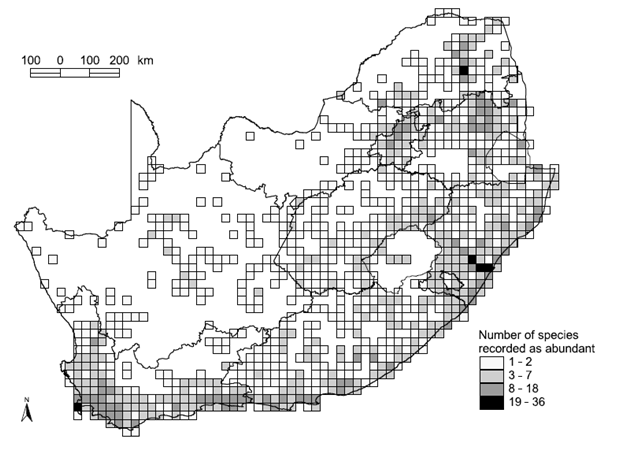
\includegraphics[scale = 0.8]{Images/SA_map}
	\caption{Distribution of alien invasive plants in South Africa (\cite{Henderson2001}).}
	\label{fig:SAmap}
\end{figure}

\clearpage
\noindent A 1996/7 survey conducted by \citet{Maitre2000} estimated that IAPs occupied approximately 10.1 million ha (or 1.736 million condensed ha) of South Africa. Combined estimates published 14 years later by \citet{Kotze2010} and \citet{VandenBerg2010} raised that figure to 1.813 million condensed ha. The annual economic cost associated with the damage inflicted by these IAPs was estimated to be approximately R6.5 billion (at 2008 inflation values) \citep{DeLange2010}. Water loss and the degradation of grazing land were the highest contributors to this figure.\newline 
One of the major groups of IAPs in both South Africa and Australia are the Cactaceae \citep{Moran1991BiologicalAfrica, Zimmermann2009, Klein2011,Paterson2011BiologicalAfrica}. The first successful biological control initiative on record for a weed was for the control of \textit{Opuntia monacantha} Haworth in India in the 1800s, and was the result of a misidentification of a \textit{Dactylopius} species \citep{Greenfield2005,Zimmermann2009}. \textit{Dactylopius ceylonicus} Green (Hemiptera: Dactylopiidae) was initially introduced to India in the belief that it was \textit{D. coccus}; a species reared for its high output of carminic acid used for the production of red dye. The insect caused such damage to \textit{O. monacantha} that the dye industry failed, but the insect continued to be used as a control agent for \textit{O. monacantha} infestations in the country, and in Sri Lanka \citep{Zimmermann2009}. Following its success in India, South Africa released \textit{D. ceylonicus} to combat \textit{O. monacantha} in 1913, which resulted in complete control of the weed within a few years and is the first intentional biological control programme on record globally \citep{lounsbury1915,Zimmermann2004BiologicalWater, Paterson2011BiologicalAfrica}. Australia followed suit and released \textit{D. ceylonicus} in 1914, which established successfully and delivered widespread control of the same weed \citep{Winston2014BiologicalWeeds.}. \\
The Dactylopiidae family (\textit{Dactylopius} Costa) is predominantly host specific to cactaceous species in the \textit{Opuntia} and \textit{Nopalea} genera \citep{DeLotto1974, Campana2015, VanDam2015}. These two cactus genera are genetically and taxonomically closely related \citep{griffith2009phylogeny}. The Dactylopiidae family is monogeneric and comprises eleven species of cactophagous insects (commonly referred to as `cochineal') \citep{Campana2015, VanDam2015}. Four \textit{Dactylopius} species are used in South Africa and Australia as biocontrol agents for invasive \textit{Opuntia} and \textit{Cylindropuntia} (Engelm.(Kuth)) cacti \citep{zachTable}. Twelve other countries around the world have released \textit{Dactylopius} species to control invasive cacti, where the impacts recorded are generally very high when establishment was successful \citep{Winston2014BiologicalWeeds.}. Many of the \textit{Dactylopius} species contain distinct genetic groups that display differential host specificities \citep{Volchansky1999, Mathenge2009,  Mathenge2010a, Mathenge2010, Jones2015, Mathenge2015}. These intraspecific groups are frequently referred to as `biotypes' in the literature, but in agreement with the criticism raised by \citet{Downie2010}, this thesis will instead use the term `lineage'. This is discussed in detail in Section \ref{sec:biotypes}. It is currently impossible to distinguish between \textit{Dactylopius} lineages using morphological characteristics \citep{Mathenge2015, jones2016host}, raising a need to address this using genetic methods. Being able to identify the species and lineages of \textit{Dactylopius} insects is fundamental to the practice of biological control of Cactaceae worldwide.  